%!TEX root = ../dokumentation.tex
\chapter{Struktur}
Die Applikation ist untergliedert in zwei Hauptbestandteile. Einen Recorder, welcher die Tonaufnahme durchführt und die erkannte Sprache in Text umwandelt, und ein Printer, welcher sich zu einer Augmenter Reality Brille verbindet und den vom Recorder erkannten Text forformatiert und darauf ausgibt. Das Bindeglied zwischen diesen beiden Komponenten ist das User Interface mit Klassenname MainActivity. Die MainActivity wird durch Usereingaben gesteuert. Sie erstellt bei bedarf neue Recorder oder Printer Instanzen, startet beziehungsweise stoppt die Aufnahme bzw die AR-Ausgabe und informiert den AR-Printer über neu verfügbare Ausgabetexte. Diese drei Komponenten werden im folgenden näher erleutert.

\section{Main Activity}
Wie bereits erwähnt ist die MainActivity das Zentrum der Applikation, ein UML-Klassendiagramm ist in XXX abgebildet.\\
Die bestandteile der MainActivity:
\begin{enumerate}
	\item Ein Spinner zur Wahl einer verfügbaren Sprachkonvertierungsoption und ein beschreibendes Textfeld
	\item Ein Spinner zur Wahl eines verfügbaren AR-Printers und ein beschreibendes Textfeld
	\item Ein Button zum Starten bzw. Stoppens einer Konvertierung
	\item Ein SideView Menü, welches Einstellungsmöglichkeiten enthält wie zum Beispiel das Festlegen der gesprochenen Sprache
	\item Eine Recorder Instanz vom Typ IRecorder. IRecorder ist ein interface, welches von allen Recorder-Implementierungen verwendet wird, um eine einheitlich API zu gewährleisten. Dieses Interface wird im Abschnitt XXX näher erleutert.
	\item Eine AR-Printer Instanz vom Typ IPrinter. Iprinter ist ebenfalls ein Interface, welches von allen AR-Printern zur Gewährleistung einer einheitlichen API implementiert wird und wird in Abschnitt XXX näher erleutert.
	\item Eine boolsche Hilfsvariable, die Auskunft darüber gibt, ob aktuell ein Konvertierungsvorgang im Gange ist.
	\item Zwei Integer-Variablen, die Auskunft über den aktuell gewählten Recorder bzw Printer geben.
\end{enumerate}
Zu 1. Und 2.:\\
Die beiden Spinner, enthalten alle aktuell supporteten Printer bzw Recorder. Der Inhalt der Spinner wird dynamisch genereiert, hierbei spielt die Klasse Constants eine tragende Rolle.\\
!!Genaueres über die initialisierung eines spinner arrays!!\\
Jedem der beiden Spinner ist eine OnItemSelectListener Instanz zugeordnet. Der OnItemSelectListener, ruft im Falle des Printer Spinners die Methode setPrinterMode(int mode, String description) und im Falle des Recorder Spinners die Methode setRecorderMode(int mode, String description) auf. Diese beiden Methoden initialisieren den gewünschten AR-Printer beziehungsweise den Recorder/Converter. Die Funktionalität dieser Methoden wird XXXX näher beschrieben.\\
Zu 3.:\\
Der OnClickListener der Buttons fragt die Hilfsvariable (7) ab und ruft abhängig von deren Wert die Methoden IRecorder.startRecording() und IPrinter.startPrinting() oder die Methode  notifyRecorderStop() der eigenen Klasse auf.\\
4. Menü: XXXX\par
Methoden der Klasse MainActivity:\\

onCreate() und initialize\_components():\\
In der onCreate()-Methode, welche beim start der Applikation ausgeführt wird, werden zunächst all Ihre bestandteile initialisiert durch die initialize\_components()-Methode.\\
setPrinterMode(int mode, String description)\\
Diese Methode prüft zuerst, ob im Moment ein Konvertierungsvorgang im Gange ist, durch das abfragen der boolschen Hilfsvariable isRecording. Im Falle einer laufenden Konvertierung wird eine Meldung ausgegeben, die den User darauf hinweißt, dass der AR-Printer während einer Konvertierung nicht gewechselt werden kann. Sonst wird nichts weiter unternommen.
Ist keine Konvertierung im Gange wird überprüft, ob der aktuelle Wert in der Hilfsvariable PRINTER\_MODE mit dem Wert des ausgewählten Printers in der übergebenen Variable mode übereinstimmt, denn auch dann muss keine weitere Aktion ausgeführt werden.\\
Wurde ein anderer Printer gewählt, als der gerade verwendete, wird die Methode generatePrinter(int mode, String description) der Klasse PrinterFactory aufgerufen. Die Methode generatePrinter prüft durch ein Switch Statement, welcher ARPrinter vom User gewünscht ist und gibt eine Instanz des gewünschten Printers and die aufrufende Methode zurück. Ist der übergebene Integer-Wert der Factory unbekannt, wird standardmäßig eine Instanz der Klasse TextPrinter erzeugt. Dieser erzeugt ein TextFeld in der MainActivity, in dem Speech to Text Conversion Ergebnisse ausgegeben werden.\\
setRecorderMode(int mode, String description):\\
Diese Methode hat den gleichen Ablauf, wie die Methode setPrinterMode(), mit dem einzigen Unterschied, dass die Methode generateRecorder der Klasse RecorderFactory aufgerufen wird, welche eine IRecorder Instanz zurück gibt. Auch die Recorder Factory hat für unbekannte Eingaben einen Standardwert. Sie gibt einen TextFieldRecorder zurück, welcher ebenfalls ein Textfeld erzeugt und die Eingaben and den gewählten AR-Printer sendet. Dieser Recorder verfehlt zwar den Sinn der Speech to Text Conversion, ist aber eine Erleichterung um die Funktionalität eines einzelnes AR-Printer Moduls zu testen.\\

receiveResult()\\
notifyStopRecord()\\

\section{Constants Klasse}
In der Klasse Constants werden globale Applikationskonstanten abgelegt. So gibt es für jede IRecorder-Implementierung einen Integer Wert, welcher den Recorder repräsentiert. Außerdem gibt es für jeden Recorder eine beschreibende String-Variable. Eine Map, welche beim start der Anwendung erzeugt wird, bringt die String-Werte mit den jeweiligen Int-Werten in Verbindung. Analog dazu besteht die selbe Struktur für Instanzen des Typs IPrinter, die unterstützten AR-Printer verwalten zu können.


\section{Interface für Augmented-Reality-Brillen-Printer}
Das Interface IPrinter definiert ein Interface, welches den gesamten Kommunikationsverlauf zwischen MainActivity und dem Augmented Reality Gerätes ermöglicht. Für den AR-Connector wurde ein Interface erzeugt um dem Erweiterbarkeitsparadigma von Software gerecht zu werden:\\
Die Klasse MainActivity ist mit einer Instanz der Klasse IPrinter, also einer Klasse, welche das Interface IPrinter implementiert, assoziiert. Innerhalb der Klasse MainActivity werden ausschließlich Methoden des Interfaces aufgerufen, keine Methoden der Implementation selbt. Aus diesem folgt, dass um ein weiteres Augmented Realitty Gerät zu unterstützen, lediglich eine einzelne neue Klasse implementiert werden muss, welche das IPrinter-Interface implementiert und der Klasse MainActivity hinzugefügt werden muss. Durch das Interface wird sichergestellt, dass alle Implementierungen über den selben Mindestmethodenumfang verfügen und Aufrufe innerhalb dieses Umfangs von allen Implementierungen verarbeitet werden können.
\paragraph{Interface-Methoden}
\begin{wrapfigure}{l}{0.6\linewidth}
	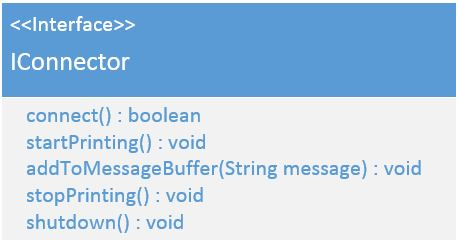
\includegraphics[width=\linewidth]{../images/iconnector.jpg}
	\caption{Interface für Augmented Reality Gerät Konnektoren}
	\label{fig:IConnector}
\end{wrapfigure}
Das Interface verlangt die im Klassendiagramm \ref{IConnector} dargestellten Methoden von seinen Erben.\\
Die Methode connect() wird nach der Initialisierung einer neuen Connector Instanz von der MainActivity aufgerufen. Diese Methode, versucht eine Verbindung zu einem Augmented Reality Gerät aufzubauen. Ihr boolscher Rückgabewert gibt Auskunft über den Erfolg des Verbindungsaufbaus.
Die startPrinting()-Methode versetzt den Connector in den Ausgabemodus. In diesem Zustand, wartet der Connector auf Nachrichten, die von der MainActivity Klasse durch die Methode addToMessageBuffer() in seinem Nachrichtenspeicher abgelegt werden und sendet diese an das Augmented Reality Gerät.\\
Die Methode stopPrinting() beendet diesen Zustand und mit der shutdown() Methode wird die Verbindung der App zum Augmented Reality Gerät beendet. Physikalisch kann die Verbindung dennoch weiterbestehen. Andere, Connectorspezifische Aktionen, welche bei Verbindungsende fällig werden, können ebenfalls in der shutdown()-Methode durchgeführt werden.
\section{Interface für Speech-To-Text-Konvertierer}
\begin{wrapfigure}{l}{0.6\linewidth}
	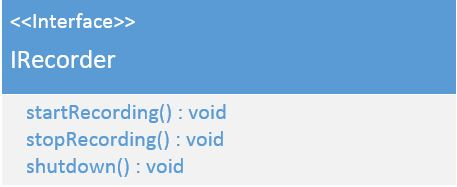
\includegraphics[width=\linewidth]{../images/IRecorder.JPG}
	\caption{Interface für Speech To Text Konvertierer}
	\label{fig:IRecorder}
\end{wrapfigure}